\chapter{부분공간, 사영 연산자, 그리고 얽힘으로서의 측정}

벨의 정리는 두 가지 질문을 남겼다. 얽힌 쌍의 한쪽이 교란되거나 흡수되거나 측정되면 얽힘은 어떻게 되는가? 그리고 정확히 무엇이 평범한 상호작용을 측정으로 바꾸는가? 답에 이르는 길은 기초 선형대수학을 거친다. 물리적 성질은 부분공간이고, 확률은 사영 연산자의 기댓값이며, 측정 장치는 대상과 얽히는 또 하나의 양자계다.

\section{도입: 얽힘, 국소성, 측정}

싱글렛이 멀리 떨어진 두 부분으로 나뉘고 그중 한쪽을 측정했다고 하자. 양자장론은 두 부분 사이에 가상 교환이 있었다고 기술해야 하는가? 먼 쪽에서는 검출 가능한 일이 일어나지 않고, 그곳에 보낼 수 있는 메시지도 전달되지 않는다. 자기장을 이용해 한쪽 스핀을 국소적으로 회전시켜 공동 상태의 구체적인 형태를 바꿀 수는 있지만, 그 국소 연산을 해도 얽힘의 양은 그대로다. 얽힘을 정량화하는 방법은 뒤에서 다룬다. 지금 중요한 점은 더 이상 상호작용하지 않는 두 계가 한쪽에만 국한된 연산만으로 공유 얽힘을 바꿀 수 없다는 것이다.

\begin{classroomqa}\lecturetimestamp{00:00:22}\audiencequestion{시공간적으로 분리된 싱글렛의 한쪽을 측정하려면 다른 쪽과 가상 교환이 있어야 하는가?}\lecturerresponse{다른 쪽에서는 검출 가능한 교환이 일어나지 않는다. 국소 연산으로 한 인자를 회전시켜 공동 상태를 표현하는 형태를 바꿀 수는 있지만, 그 연산만으로는 메시지를 보내거나 두 부분 사이에 공유된 얽힘을 바꿀 수 없다.}\end{classroomqa}

이 때문에 무엇을 얽힘의 상대 계로 볼지 더 폭넓게 생각해야 한다. 얽힌 쌍의 한쪽이 블랙홀에 빠지더라도 다른 쪽과의 얽힘이 사라지는 것은 아니다. 그 입자는 블랙홀의 자유도와 얽히고, 블랙홀이 증발한 뒤에는 방출된 복사와 얽힌다. 이와 같은 생각을 적용하는 데 블랙홀은 필요하지 않다. 얽힌 쌍의 한쪽을 욕조에 빠뜨려 물과 격렬하게 섞이게 해 보자. 다체 상태 속에서 그 입자의 개별 정체성은 사라질 수 있지만, 멀리 있는 입자는 여전히 욕조 전체와 얽혀 있고, 결국 빠져나가는 수증기와도 얽힌다.

이것은 얽힘이 지속된다는 이야기만은 아니다. 가역성에 관한 이야기이기도 하다. 상호작용으로 얽힘을 만들 수 있다면, 원칙적으로 상호작용으로 얽힘을 되돌릴 수도 있다. 얽힘을 풀 수는 있지만, 계들이 다시 접촉해 상호작용해야만 가능하다. 한 방향으로 일어날 수 있는 일은 반대 방향으로도 일어날 수 있다.

\begin{classroomqa}\lecturetimestamp{00:04:45}\audiencequestion{얽힌 쌍의 두 스핀을 모두 측정하면 전자들은 계속 얽혀 있는가? 측정 한 번만으로 이미 얽힘이 풀릴 수도 있는가?}\lecturerresponse{측정으로 둘 사이의 얽힘을 없앨 수 있으며, 측정 한 번이면 충분할 수도 있다. 단순히 파동 묶음의 붕괴라고 단언하는 대신 그 말이 무엇을 뜻하는지 알려면, 관측을 계와 기록 장치 사이의 상호작용으로 기술해야 한다.}\end{classroomqa}

이 질문이 우리가 다룰 과제를 정한다. 관측, 파동 묶음의 붕괴, 얽힘을 연결하는 것이다. 하지만 거기에 앞서, 필요한 만큼의 기초적인 도구만으로 부분공간과 사영 연산자를 더 명료하게 설명할 필요가 있다.

\section{차원, 선형 종속성, 정규직교 기저}

그러므로 우선 브라, 켓, 내적을 갖춘 유한 차원 벡터 공간을 다룬다. 서스킨드는 가능한 한 기초적인 방식으로 시작한다. 열벡터의 성분을 세어 차원을 정의하지 않는다. 차원을 추상적으로 정의한다. 벡터 공간의 차원이란 그 안에서 찾을 수 있는 선형 독립 벡터의 최대 개수다.

따라서 벡터들의 모임 \(\{|v_i\rangle\}\)은 다음 관계에서 \begin{equation}
\sum_i c_i |v_i\rangle = 0
\end{equation} 모든 계수 \(c_i\)가 영이 되는 경우 선형 독립이다. 달리 말해, 어느 벡터도 나머지 벡터들의 선형 결합으로 나타낼 수 없다.

여기서 직교성과 선형 독립성은 서로 다르다는 점이 중요하다. 삼차원 공간에는 서로 전혀 직교하지 않으면서도 선형 독립인 벡터 세 개가 있을 수 있다. 중요한 것은 그중 하나를 나머지 두 벡터로 만들 수 있는지 여부다. 반면 이차원 평면에서는 그 평면 안의 세 번째 벡터가 앞의 두 벡터에 선형 종속일 수밖에 없다.

\begin{figure}[htbp]\centering
\includegraphics[width=0.56\textwidth]{lecture_06_figure_02.png}\caption{칠판에 그린 세 벡터. 강의에서는 이 그림으로 직교성과 선형 독립성을 구분한 뒤, 평면에서 세 번째 벡터가 앞의 두 벡터에 종속됨을 강조한다.}\lectureframe{00:09:35}\end{figure}

\begin{figure}[htbp]\centering
\begin{tikzpicture}[scale=1.2]
\draw[->] (0,0) -- (2.3,0);
\draw[->] (0,0) -- (2.0,2.0);
\draw[->] (0.35,0.95) -- (1.05,1.45);
\fill (0,0) circle (1.2pt);
\end{tikzpicture}\caption{칠판 그림을 간결하게 재구성한 것. 이 장면만으로는 구체적인 계수 관계를 정할 수 없다. 기하학적 요점은 이차원 평면의 세 번째 벡터는 선형 독립일 수 없다는 것이다.}\end{figure}

그림의 요점이 바로 이것이다. 공간의 차원이 이라면 선형 독립 벡터의 최대 개수는 둘이다. 공간의 차원이 삼이라면 최대 개수는 셋이다. 더 일반적으로 공간의 차원이 \(d\)이면, 내적이 주어졌을 때 그 공간을 생성하는 서로 직교하는 단위 벡터 \(d\)개를 찾을 수 있다. 이것들이 기저 벡터다. 서스킨드는 여기서 그 정리를 증명하지 않겠다고 분명히 말한다. 그가 강조하려는 결론은 이것이다. 그러한 기저가 있으면 공간의 모든 벡터를 그 기저 벡터들의 선형 결합으로 전개할 수 있다.

\begin{classroomqa}\lecturetimestamp{00:10:58}\audiencequestion{공간적 자유도의 개수는 상태 공간의 차원과 같은가?}\lecturerresponse{아니다. 방 안에서 움직이는 입자는 공간 좌표가 세 개지만 서로 직교하는 양자 상태는 엄청나게 많다. 배치 공간의 차원과 힐베르트 공간의 차원은 서로 다른 개념이다. 유한 차원 예제는 논리를 명료하게 보여 주기 위해서만 사용한다.}\end{classroomqa}

\section{기저 전개, 다이애드, 항등 연산자의 분해}

이제 \(\{|n\rangle\}\)을 정규직교 기저로 잡자. 여기서 \(n=1,\dots,d\)이다. 이 대목의 칠판 설명은 특히 명료하고 간결하다.

\begin{figure}[htbp]\centering
\includegraphics[width=0.62\textwidth]{lecture_06_figure_03.png}\caption{정규직교 기저와 임의의 상태의 전개.}\lectureframe{00:14:15}\end{figure}

다음과 같이 쓴다. \begin{align}
\langle m|n\rangle &= \delta_{mn}, \\
|\psi\rangle &= \sum_n a_n |n\rangle.
\end{align} 여기서 \(\delta_{mn}\)는 크로네커 델타다. \(m=n\)일 때는 \(1\)이고, 그렇지 않을 때는 \(0\)이다.

\paragraph{유도}계수는 기저에 사영해 구한다. 왼쪽에서 \(\langle m|\)를 곱하면 \begin{align}
\langle m|\psi\rangle
  &= \sum_n a_n \langle m|n\rangle \\
  &= \sum_n a_n \delta_{mn} \\
  &= a_m.
\end{align}가 된다. 따라서 계수는 간단히 \begin{equation}
a_m = \langle m|\psi\rangle.
\end{equation}와 같다. 계수는 보통의 복소수이므로 켓의 어느 쪽에 놓아도 값은 변하지 않는다.

이 계수를 전개식에 다시 대입하면 \begin{equation}
|\psi\rangle = \sum_n |n\rangle \langle n|\psi\rangle.
\end{equation}을 얻는다. 여기서 \(|n\rangle\langle n|\), 더 일반적으로 \(|a\rangle\langle b|\)를 연산자로 해석해야 한다는 생각이 나온다. 바로 이것이 다음 단계다. 다이애드는 다음과 같이 작용한다. \begin{equation}
\bigl(|a\rangle\langle b|\bigr)|\psi\rangle = \langle b|\psi\rangle\,|a\rangle.
\end{equation} 브라는 복소수를 뽑아내고, 켓은 그 결과에 해당하는 방향을 제공한다. 이는 벡터에서 연산자로 나아가는 서스킨드의 간단한 방법이다.

앞의 전개식을 연산자 관점에서 보자. \begin{equation}
|\psi\rangle = \left(\sum_n |n\rangle\langle n|\right)|\psi\rangle
\end{equation}가 모든 \(|\psi\rangle\)에 대해 성립하므로 괄호 안의 연산자는 항등 연산자여야 한다. \begin{equation}
\sum_n |n\rangle\langle n| = I.
\end{equation} 이것이 항등 연산자의 분해다.

\begin{figure}[htbp]\centering
\includegraphics[width=0.60\textwidth]{lecture_06_figure_07.png}\caption{칠판에 완성된 항등 연산자 분해.}\lectureframe{00:18:30}\end{figure}

\begin{classroomqa}\lecturetimestamp{00:18:39}\audiencequestion{항등 연산자 분해에 나오는 벡터들은 기저여야 하는가?}\lecturerresponse{그렇다. 유도 과정은 정규화와 상호 직교성을 모두 사용하며, 합은 완비 기저 전체에 대해 취해야 한다. 임의의 벡터 모임으로는 항등 연산자를 분해할 수 없다.}\end{classroomqa}

항등 연산자 자체가 공간 전체로의 사영 연산자다. 모든 벡터는 \(I\)의 고유벡터이고, 모든 고윳값은 \(+1\)이다.

\begin{classroomqa}\lecturetimestamp{00:19:14}\audiencequestion{항등 연산자의 분해는 모든 벡터의 고윳값이 일이라고 말하는가?}\lecturerresponse{그렇다. 항등 연산자의 경우에는 모든 벡터가 그 고유벡터이고 모든 상태에 대해 \(I|\psi\rangle=|\psi\rangle\)가 성립한다는 점에서 특별하다.}\end{classroomqa}

\section{부분공간으로서의 물리량과 사영 연산자}

이 도구들을 갖춘 뒤, 강의는 핵심 개념을 바로잡는다. \(k=\lambda\)와 같은 물리량은 일반적으로 벡터 하나를 뜻하지 않는다. 하나의 부분공간 전체를 뜻한다.

\(k\)를 에르미트 관측량이라 하고, \begin{equation}
k|A\rangle = \lambda |A\rangle, \qquad
k|B\rangle = \lambda |B\rangle,
\end{equation}라고 하자. 여기서 \(|A\rangle\)와 \(|B\rangle\)는 선형 독립이다. 그러면 임의의 선형 결합도 같은 고윳값을 갖는다. \begin{align}
k\bigl(\alpha|A\rangle+\beta|B\rangle\bigr)
  &= \alpha k|A\rangle + \beta k|B\rangle \\
  &= \alpha \lambda |A\rangle + \beta \lambda |B\rangle \\
  &= \lambda\bigl(\alpha|A\rangle+\beta|B\rangle\bigr).
\end{align} 그러므로 \(\lambda\)에 해당하는 고유공간은 덧셈과 스칼라 곱에 대해 닫혀 있다. 즉 벡터 부분공간이다.

강의에서 처음 드는 구체적인 예는 두 스핀 계다. 상태 \begin{equation}
|ud\rangle,\qquad |uu\rangle
\end{equation}는 두 번째 스핀의 값은 서로 다르지만 첫 번째 스핀의 값은 같다. 두 상태 모두 첫 번째 스핀이 위쪽이다. 따라서 두 상태는 첫 번째 스핀에서 \(\sigma_3=+1\)인 부분공간을 생성한다.

\begin{figure}[htbp]\centering
\includegraphics[width=0.46\textwidth]{lecture_06_figure_04.png}\caption{첫 번째 스핀이 위쪽인 두 스핀 상태.}\lectureframe{00:23:27}\end{figure}

기억해야 할 요점은 이것이다. 물리량이 반드시 상태 하나에 대응하는 것은 아니다. 같은 고윳값을 갖는 상태들의 집합 전체에 대응한다.

칠판에서 잠시 나타나는 표기상의 혼동을 피하기 위해, 특정 고유벡터에는 대문자 \(A,B,\dots\)를 쓰고, 고유부분공간의 정규직교 기저를 순회하는 합의 첨자에는 소문자 \(a,b,\dots\)를 쓰겠다. \(\{|a\rangle\}\)가 부분공간 \(k=\lambda\)의 기저라면, 그 부분공간으로의 사영 연산자는 다음과 같다. \begin{equation}
\Pi_{k=\lambda}=\sum_a |a\rangle\langle a|.
\end{equation} 이것은 부분공간에만 제한한 항등 연산자다. \(|\psi\rangle\)가 이미 그 부분공간에 있으면 사영 연산자는 이를 그대로 돌려준다. \(|\psi\rangle\)가 부분공간 밖에 걸쳐 있으면 직교하는 나머지 성분을 버리고 내부 성분만 남긴다.

\section{확률 공리, 양립 가능한 물리량, 그리고 벨 정리 복습}

물리량을 부분공간으로 다시 이해하고 나면 확률 공리는 가장 간결한 형태를 취한다. \(|\psi\rangle\)가 정규화되어 있을 때, 그 상태가 물리량 \(k=\lambda\)을 갖는 확률은 다음과 같다. \begin{equation}
P(k=\lambda)=\langle\psi|\Pi_{k=\lambda}|\psi\rangle.
\end{equation}

\begin{figure}[htbp]\centering
\includegraphics[width=0.58\textwidth]{lecture_06_figure_05.png}\caption{\(k=\lambda\)의 고유부분공간으로의 사영 연산자. 칠판의 표기는 다음 단계를 이미 예고한다. 사영 연산자를 \(\langle\psi|\)와 \(|\psi\rangle\) 사이에 끼워 넣는다.}\lectureframe{00:31:09}\end{figure}

사영 연산자를 다이애드 형태로 대입하면 \begin{align}
P(k=\lambda)
  &= \left\langle \psi \left| \sum_a |a\rangle\langle a| \right| \psi \right\rangle \\
  &= \sum_a \langle\psi|a\rangle\langle a|\psi\rangle \\
  &= \sum_a |\langle a|\psi\rangle|^2.
\end{align}을 얻는다. 이는 강의에서 설명한 그대로다. 해당 물리량에 대한 총확률은 그 물리량이 나타날 수 있는 서로 직교하는 모든 방식의 확률을 더한 것이다.

두 스핀 계에서 첫 번째 스핀이 위쪽인 상태와 관련된 부분공간은 \(|uu\rangle\)와 \(|ud\rangle\)가 생성하므로 \begin{equation}
\Pi_{\sigma_3=+1}=|uu\rangle\langle uu|+|ud\rangle\langle ud|.
\end{equation}이다. 강의에서는 두 번째 스핀에 작용하는 항등 연산자를 생략해 \begin{equation}
\Pi_{\sigma_3=+1}=\frac{1+\sigma_3}{2},
\end{equation}라고 줄여 쓰기도 한다.

\begin{classroomqa}\lecturetimestamp{00:33:04}\audiencequestion{관측량, 물리량, 사영 연산자의 차이는 무엇인가?}\lecturerresponse{관측량은 에르미트 연산자 \(k\)다. 물리량 \(k=\lambda\)는 그 고유부분공간으로 나타내며, \(k\)를 측정하면 반드시 \(\lambda\)가 나온다는 뜻이다. 사영 연산자 \(\Pi_{k=\lambda}\)는 그 부분공간을 분리해 내며, 그 기댓값은 해당 물리량이 나타날 확률을 준다.}\end{classroomqa}

\begin{classroomqa}\lecturetimestamp{00:34:07}\audiencequestion{축퇴 고유벡터 \(A\)와 \(B\)는 이미 서로 직교해야 하는가? 그리고 이 벡터들은 공간 전체의 기저인가?}\lecturerresponse{원래의 고유벡터들은 서로 직교할 필요가 없지만, 그 고유부분공간 안에서는 언제나 정규직교 기저를 선택할 수 있다. 그 기저는 해당 부분공간의 기저일 뿐이다. 전체 공간을 생성하려면 추가로 직교하는 방향들이 필요하다. 부분공간의 각 기저 벡터에 사영한 뒤 그 결과를 더하면 부분공간으로의 사영이 된다.}\end{classroomqa}

\begin{classroomqa}\lecturetimestamp{00:35:33}\audiencequestion{\(a\)라는 기호는 \(k|A\rangle=\lambda|A\rangle\)에서 쓰인 \(a\)와 사영 연산자에서 합을 취하는 첨자와 같은 뜻인가?}\lecturerresponse{아니다. 앞의 기호는 특정 고유벡터를 나타내지만, 합의 아래에 있는 첨자는 고유부분공간의 정규직교 기저에 속하는 모든 벡터를 순회한다. 표기를 구분하면 특정한 표지를 합의 더미 첨자로 오해하지 않게 된다.}\end{classroomqa}

\begin{classroomqa}\lecturetimestamp{00:37:15}\audiencequestion{사영 연산자 식에 나오는 내적은 확률인가, 확률 진폭인가?}\lecturerresponse{각각의 \(\langle a|\psi\rangle\)는 진폭이다. 여기에 복소켤레를 곱하면 확률이 되고, \(k=\lambda\)을 실현하는 서로 직교하는 여러 방식의 확률을 합하면 해당 물리량의 총확률이 된다.}\end{classroomqa}

이어서 강의는 물리량들을 결합하는 방법을 묻는다. 서로 양립하고 사영 연산자 \(P_k\)와 \(P_\ell\)로 나타내는 두 물리량이 있다고 하자. 강의의 표현을 따르면 AND 명제는 곱으로 나타낸다. \begin{equation}
\Pi_{k=\lambda\,\wedge\,\ell=\mu}=P_kP_\ell=P_\ell P_k.
\end{equation} 논리는 간단하다. \(P_k|\psi\rangle\)는 \(k=\lambda\) 부분공간에 속한다. 연산자들이 서로 가환하므로 \(P_\ell P_k|\psi\rangle=P_kP_\ell|\psi\rangle\)이고, 따라서 같은 벡터는 \(\ell=\mu\) 부분공간에도 속한다. 그러므로 두 연산자의 곱은 두 물리량이 동시에 성립하는 부분공간으로 사영한다. 이에 해당하는 확률은 \begin{equation}
P(k=\lambda,\ell=\mu)=\langle\psi|P_kP_\ell|\psi\rangle.
\end{equation}이다.

이 논증의 첫 단계는 따로 살펴볼 만하다. 임의의 상태에 대해 \begin{equation}
k\bigl(P_k|\psi\rangle\bigr)=\lambda P_k|\psi\rangle,
\end{equation}이므로 \(P_k|\psi\rangle\)는 \(k=\lambda\) 고유부분공간에 속한다. \(P_k\)와 \(P_\ell\)가 가환하면 곱을 어느 사영 연산자를 왼쪽에 두든 같은 형태로 쓸 수 있다. 따라서 그 결과는 두 부분공간 모두에 속한다.

\begin{figure}[htbp]\centering
\includegraphics[width=0.44\textwidth]{lecture_06_figure_06.png}\caption{고유부분공간에 속하는 벡터로서의 사영된 상태.}\lectureframe{00:41:57}\end{figure}

\begin{figure}[htbp]\centering
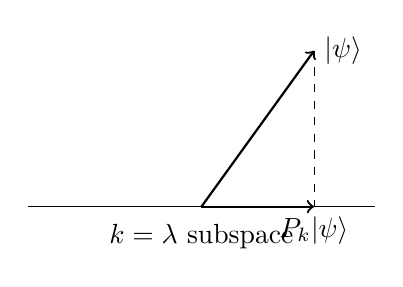
\begin{tikzpicture}[scale=1.1]
\draw (-2,0) -- (2,0);
\draw[->,thick] (0,0) -- (1.3,1.8) node[right] {$|\psi\rangle$};
\draw[dashed] (1.3,1.8) -- (1.3,0);
\draw[->,thick] (0,0) -- (1.3,0) node[below] {$P_k|\psi\rangle$};
\node at (0,-0.35) {$k=\lambda$ subspace};
\end{tikzpicture}\caption{\(k=\lambda\) 고유부분공간으로 임의의 벡터를 사영하는 모습.}\end{figure}

\begin{figure}[htbp]\centering
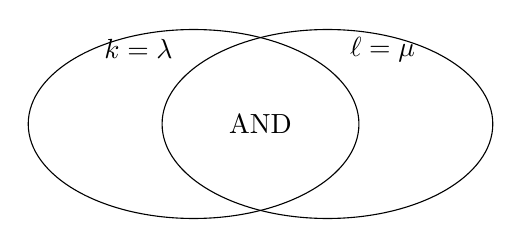
\begin{tikzpicture}[scale=1.0]
\draw (0,0) ellipse (2.1 and 1.2);
\draw (1.7,0) ellipse (2.1 and 1.2);
\node at (-0.7,0.95) {$k=\lambda$};
\node at (2.4,0.95) {$\ell=\mu$};
\node at (0.85,0) {AND};
\end{tikzpicture}\caption{가환 사영 연산자의 AND 명제 뒤에 있는 교차 부분공간 그림의 재구성.}\end{figure}

\begin{figure}[htbp]\centering
\includegraphics[width=0.66\textwidth]{lecture_06_figure_08.png}\caption{가환 사영 연산자가 동시 고유부분공간을 선택한다는 칠판 논증.}\lectureframe{00:45:20}\end{figure}

\begin{classroomqa}\lecturetimestamp{00:44:42}\audiencequestion{두 물리량이 동시에 성립하는 부분공간은 고전 논리에서의 교집합과 같은가?}\lecturerresponse{그렇다. 가환 사영 연산자에서 \(P_kP_\ell\)는 두 고유부분공간의 교집합으로 사영한다. 그 교집합이 영벡터만 포함한다면 두 물리량을 모두 갖는 영이 아닌 상태는 없다.}\end{classroomqa}

완전성을 위해, 양립 가능한 OR 부분공간으로의 사영 연산자는 다음과 같다. \begin{equation}
P_{k\lor\ell}=P_k+P_\ell-P_kP_\ell .
\end{equation} 두 대안이 서로 배타적이면 \(P_kP_\ell=0\)이므로 식은 합 \(P_k+P_\ell\)으로 단순해진다. 두 부분공간이 겹칠 때는 교집합을 두 번 세지 않도록 이 뺄셈이 반드시 필요하다.

이어 양립 가능성은 물리적 예와 연결된다. 두 스핀 계에서 첫 번째 스핀의 임의의 성분 \(\sigma_i\)은 두 번째 스핀의 임의의 성분 \(\tau_j\)와 가환한다. \begin{equation}
[\sigma_i,\tau_j]=0.
\end{equation} 반면 같은 스핀의 서로 다른 성분들은 가환하지 않는다. \begin{equation}
[\sigma_1,\sigma_3]\neq 0.
\end{equation} 그렇기 때문에 서로 떨어진 두 스핀에서는 각 스핀의 한 성분씩 측정할 수 있지만, 한 스핀의 서로 다른 두 성분을 동시에 측정할 수는 없다.

\begin{classroomqa}\lecturetimestamp{00:46:12}\audiencequestion{양립 가능한 관측량의 구체적인 예에는 무엇이 있는가?}\lecturerresponse{첫 번째 스핀에 작용하는 연산자는 모두 두 번째 스핀에 작용하는 모든 연산자와 가환한다. 서로 다른 텐서 인자에 작용하기 때문이다. 위치 성분 \(x,y,z\)도 서로 양립하는 한 묶음이다. 반면 같은 스핀의 서로 다른 두 성분이나 위치와 그 켤레 운동량은 가환하지 않는다.}\end{classroomqa}

\begin{classroomqa}\lecturetimestamp{00:47:26}\audiencequestion{부분계는 반드시 다른 입자를 뜻하는가?}\lecturerresponse{아니다. 독립적으로 지정된 자유도들의 집합을 뜻한다. 서로 다른 입자는 가장 단순한 텐서 인자를 이루지만, 연산자 구조가 허용하면 한 입자의 서로 다른 자유도도 따로 다룰 수 있다.}\end{classroomqa}

\begin{classroomqa}\lecturetimestamp{00:48:37}\audiencequestion{서로 다른 부분계의 많은 연산자가 가환한다면, 간단한 비양립 쌍은 무엇인가?}\lecturerresponse{같은 스핀의 두 성분이 대표적인 예다. \(\sigma_1\)와 \(\sigma_3\)는 가환하지 않으므로 어떤 측정 장치도 두 값을 동시에 확정된 값으로 부여할 수 없다. 행렬의 교환자가 영이 아닌지가 대수적인 판정 기준이다.}\end{classroomqa}

이제 서스킨드는 벨 정리를 다시 살펴본다. 앞 강의의 계산을 반복하는 대신, 새로운 표현으로 그 논리를 다시 세운다. 확률로 쓴 고전적 부등식은 다음과 같다. \begin{equation}
P(A\wedge \neg B)+P(B\wedge \neg C)\ge P(A\wedge \neg C).
\end{equation} 이것은 양자역학의 정리가 아니라 고전적인 집합 논리의 정리다. 싱글렛 상태에서는 공통 축을 기준으로 스핀들이 반대 방향이므로, 첫 번째 스핀에 대한 NOT 명제를 두 번째 스핀에 대응하는 긍정 명제로 바꿔 쓸 수 있다. 그러면 부등식을 두 스핀 계의 공동 성질에 관한 명제로 다시 쓸 수 있다.

건드리지 않는 인자에 작용하는 항등 연산자를 생략하면, 강의에서 쓰는 단일 물리량의 사영 연산자는 다음과 같다. \begin{equation}
\frac{1+\sigma_3}{2},\qquad
\frac{1+\frac{\tau_1+\tau_3}{\sqrt2}}{2},\qquad
\frac{1+\frac{\sigma_1+\sigma_3}{\sqrt2}}{2},\qquad
\frac{1+\tau_1}{2}.
\end{equation} 따라서 관련된 세 개의 공동 사영 연산자는 다음과 같다. \begin{align}
\Pi_1 &= \frac{1+\sigma_3}{2}\,\frac{1+\frac{\tau_1+\tau_3}{\sqrt2}}{2}, \\
\Pi_2 &= \frac{1+\frac{\sigma_1+\sigma_3}{\sqrt2}}{2}\,\frac{1+\tau_1}{2}, \\
\Pi_3 &= \frac{1+\sigma_3}{2}\,\frac{1+\tau_1}{2}.
\end{align}

\begin{figure}[htbp]\centering
\includegraphics[width=0.68\textwidth]{lecture_06_figure_09.png}\caption{한 스핀의 사영 연산자들의 곱으로 쓴 세 가지 분석기 설정.}\lectureframe{01:01:45}\end{figure}

강의에서는 친숙한 정규화 전 형태의 칠판 표기로 싱글렛을 나타낸다. \begin{equation}
|\Psi_{\mathrm{singlet}}\rangle \propto |ud\rangle-|du\rangle.
\end{equation} 비례 기호만으로 여기서는 충분하다. 논리에 중요한 것은 상태 자체, 특히 상대 부호이지 전체 정규화 인자는 아니다. 싱글렛 상태에서 \(\langle \Pi_3\rangle\)에 대한 \(\langle \Pi_1\rangle+\langle \Pi_2\rangle\)의 값을 계산하면 앞 강의에서 얻은 위배가 나온다. 서스킨드가 말로 강조하는 핵심 결론은 이것이다. 양자역학은 위장한 고전적 집합론이 아니다.

\begin{classroomqa}\lecturetimestamp{00:52:31}\audiencequestion{스핀 위쪽 상태와 아래쪽 상태가 서로 직교한다면, 마이너스 부호는 한 켓이 다른 켓의 음수라는 뜻인가?}\lecturerresponse{아니다. \(|u\rangle\)와 \(|d\rangle\)는 서로 다른 직교 벡터다. 상대 부호는 \(|ud\rangle-|du\rangle\)와 같은 중첩 상태에 붙으며, 그 물리적 성질을 바꿀 수 있다. 전체 상태에 곱해지는 전체 부호만 물리적으로 무관하다.}\end{classroomqa}

\begin{classroomqa}\lecturetimestamp{00:53:06}\audiencequestion{모든 양자 상태와 모든 물리량 선택에서 벨 부등식이 위배되는가?}\lecturerresponse{아니다. 많은 상태와 여러 축 선택에서는 특정 벨 부등식을 만족한다. 위배 여부는 상태와 선택한 관측량 모두에 달려 있다. 중간 각도와 마지막 각도를 바꾸면 이 검사가 비고전적 상관관계를 드러내는지가 달라진다.}\end{classroomqa}

\begin{classroomqa}\lecturetimestamp{01:02:47}\audiencequestion{특정 상태가 이 벨 부등식을 위배하거나 우연히 만족하면 무엇을 결론 내릴 수 있는가?}\lecturerresponse{부등식의 위배는 관측된 통계가 유도 과정에서 사용한 고전적 집합 논리로는 나올 수 없음을 증명한다. 선택한 부등식 하나를 만족한다고 해서 그 상태가 고전적이라는 뜻은 아니다. 다른 물리량을 선택하면 위배가 드러날 수도 있다.}\end{classroomqa}

\section{벨 정리 이후의 국소성}

사영 연산자 계산은 단순한 기호 놀이가 아니다. 싱글렛 바닥 상태에서 상관된 쌍을 반복해서 준비한 뒤 두 입자를 서로 떨어뜨리고, 동일하게 준비된 앙상블을 세 개의 큰 집단으로 나눈다고 하자. 첫 번째 집단에서는 \(0^\circ\)와 \(45^\circ\) 설정을, 두 번째에서는 \(45^\circ\)와 \(90^\circ\) 설정을, 세 번째에서는 \(0^\circ\)와 \(90^\circ\) 설정을 측정한다. 각 집단에서 얻은 빈도로 부등식에 등장하는 세 확률을 추정한다.

\begin{classroomqa}\lecturetimestamp{01:04:30}\audiencequestion{세 벨 확률은 실제 실험실에서 어떤 배치를 나타내는가?}\lecturerresponse{장치가 동일하게 준비된 얽힌 쌍을 많이 만들고 두 입자를 떨어진 분석기로 보낸다. 쌍들을 세 앙상블로 나눈 뒤 각 앙상블에서 해당하는 두 분석기 방향을 사용한다. 공동 측정 결과를 세어 각 확률을 추정한다. 전하를 띤 입자와 반입자는 장으로 분리할 수 있지만, 실제 벨 실험에서는 흔히 광자를 사용한다.}\end{classroomqa}

\begin{classroomqa}\lecturetimestamp{01:08:00}\audiencequestion{고전적인 집합 증명은 하나의 모집단을 사용했다. 어떻게 서로 따로 측정한 세 앙상블로 그 증명을 검증할 수 있는가?}\lecturerresponse{이 부등식은 도수뿐 아니라 확률에 관한 명제이기도 하다. 세 표본을 모두 같은 준비 절차에서 얻으면 상대도수로 공통 앙상블 하나의 세 확률 분포를 추정할 수 있다. 동일한 준비는 반드시 필요한 가정이다.}\end{classroomqa}

이 벨 정리 복습은 방 안에 여전히 남아 있는 물리적 의문으로 곧바로 이어진다. 상관관계가 실재한다면 왜 그것으로 신호를 보낼 수 없을까?

\begin{classroomqa}\lecturetimestamp{01:09:41}\audiencequestion{얽힌 상관관계로 광속보다 빠른 메시지를 보낼 수 없는 이유는 무엇인가?}\lecturerresponse{각 측정 지점에서 따로 보면 통제할 수 없는 무작위 결과만 관측된다. 상관관계는 두 기록을 통상의 고전적 통신 채널로 비교할 때에만 드러난다. 하지만 결정적인 벨 실험에서는 두 지점 사이에 빛 신호가 제때 오갈 수 없도록 측정 선택과 검출 시점을 정한다. 그럼으로써 공동 통계를 만들어 내는 국소적 통신 메커니즘을 배제한다.}\end{classroomqa}

빛 신호가 장치들 사이를 오갈 만큼 시간이 충분히 지나면, 상관관계 자체가 상대성 이론과 모순되는 것은 아니다. 단지 알아차리지 못한 통상의 영향이 발견되었을 수도 있다. 결정적인 실험은 이런 가능성을 차단한다. 벨의 표현을 따르면, 상관관계를 재현하는 숨은 변수 설명은 비국소적이어야 한다. 그러나 비국소적 의존성은 통제 가능한 초광속 메시지와 같은 것이 아니다.

\begin{classroomqa}\lecturetimestamp{01:12:18}\audiencequestion{각운동량 보존은 이 논증에 반드시 필요한가?}\lecturerresponse{아니다. 스핀은 편리한 이준위 모형일 뿐, 반드시 필요한 요소는 아니다. 필요한 얽힘 상태와 서로 다른 측정 기저를 갖춘 이준위 계의 쌍이라면 같은 논리 구조를 나타낼 수 있다.}\end{classroomqa}

이 논의로 강의가 끝나는 것은 아니다. 다음 주제로 넘어갈 길을 열어 준다. 벨 정리는 양자역학이 고전 논리가 아님을 보여 주었다. 하지만 다음 질문은 다르다. 조작적·수학적으로 측정이란 무엇이며, 간섭에 관한 이야기에는 어떻게 들어오는가?

\section{유한 상태 이중 슬릿, 간섭, 그리고 얽힘으로서의 측정}

이제 강의에서 모형이 바뀐다. 서스킨드는 이중 슬릿 실험으로 넘어가면서도, 연속적인 파동역학의 전체 도구를 가져오지 않고 같은 벡터 공간 기법을 쓸 수 있도록 문제를 유한 상태 문제로 단순화한다. 사실상 이것은 여전히 이중 슬릿 실험이지만, 적은 수의 기저 상태만 남도록 단순화한 것이라고 말한다.

근원 상태 \(|0\rangle\), 두 슬릿 상태 \(|1\rangle\)와 \(|-1\rangle\), 그리고 스크린 상태들의 집합 \(|n\rangle\)가 있다. 서로 다른 스크린 위치는 서로 다른 배열이므로 이들 \(|n\rangle\)는 정규직교한다. 이 대목에서는 정규화를 엄밀히 다루지 않겠다고 강의에서 명시한다. 유니터리성은 뒤로 미룬다. 지금 중요한 것은 선형성이다.

\begin{figure}[htbp]\centering
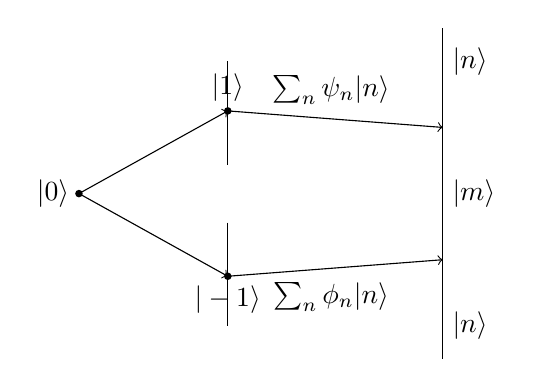
\begin{tikzpicture}[scale=1.05]
\fill (0,0) circle (1.3pt);
\node[left] at (0,0) {$|0\rangle$};

\draw (1.8,1.6) -- (1.8,0.35);
\draw (1.8,-0.35) -- (1.8,-1.6);
\fill (1.8,1) circle (1.3pt);
\fill (1.8,-1) circle (1.3pt);
\node[above] at (1.8,1) {$|1\rangle$};
\node[below] at (1.8,-1) {$|-1\rangle$};

\draw (4.4,2.0) -- (4.4,-2.0);
\node[right] at (4.4,1.6) {$|n\rangle$};
\node[right] at (4.4,0.0) {$|m\rangle$};
\node[right] at (4.4,-1.6) {$|n\rangle$};

\draw[->] (0,0) -- (1.8,1);
\draw[->] (0,0) -- (1.8,-1);
\draw[->] (1.8,1) -- (4.4,0.8);
\draw[->] (1.8,-1) -- (4.4,-0.8);

\node at (3.05,1.25) {$\sum_n \psi_n |n\rangle$};
\node at (3.05,-1.25) {$\sum_n \phi_n |n\rangle$};
\end{tikzpicture}\caption{이중 슬릿 실험의 유한 상태 모형: 근원 상태 \(|0\rangle\), 두 슬릿 상태 \(|1\rangle\)와 \(|-1\rangle\), 그리고 스크린 기저 \(|n\rangle\).}\end{figure}

\begin{figure}[htbp]\centering
\includegraphics[width=0.68\textwidth]{lecture_06_figure_10.png}\caption{선형 시간발전 규칙 \(A\to A'\), \(B\to B'\)과 나란히 나타낸 유한 위치 격자.}\lectureframe{01:18:00}\end{figure}

대칭성에 따라 근원 상태는 두 슬릿 상태의 진폭이 같은 중첩 상태로 시간에 따라 변한다. \begin{equation}
|0\rangle \longrightarrow |1\rangle+|-1\rangle.
\end{equation} 이제 위쪽 슬릿 상태가 다음 상태로 변한다고 하자. \begin{equation}
|1\rangle \longrightarrow \sum_n \psi_n |n\rangle,
\end{equation} 아래쪽 슬릿 상태는 다음 상태로 변한다고 하자. \begin{equation}
|-1\rangle \longrightarrow \sum_n \phi_n |n\rangle.
\end{equation} 여기서 화살표는 같은 순간의 상태 사이의 등호가 아니라 시간발전을 뜻한다. 선형성에 따라 \begin{equation}
|1\rangle+|-1\rangle \longrightarrow \sum_n (\psi_n+\phi_n)|n\rangle.
\end{equation}가 성립한다. 이것이 핵심 규칙이다. 확률을 구하기 전에 진폭을 먼저 더한다.

\begin{classroomqa}
\lecturetimestamp{01:21:59}
\audiencequestion{슬릿 상태 \(|1\rangle\)는 어떻게 정수로도 표기되는 상태 \(n\)들로 변할 수 있나요? 이 켓들은 같은 장소와 같은 시간에 있는 건가요?}
\lecturerresponse{여기서 표기는 서로 다른 시간 단면을 가리킵니다. \(|1\rangle\)는 위쪽 슬릿에 있는 전자를 나타내고, 오른쪽의 \(|n\rangle\)는 스크린 위의 가능한 이후 위치를 나타냅니다. 화살표는 시간에 따른 상태의 변화를 뜻하며, 동시에 존재하는 배치들이 서로 같다는 뜻은 아닙니다.}
\end{classroomqa}

\begin{classroomqa}
\lecturetimestamp{01:25:30}
\audiencequestion{진폭은 정규화되어야 하나요? 물리적 단위를 갖나요?}
\lecturerresponse{완전한 시간 진화는 전체 확률을 보존해야 합니다. 이것이 유니터리성입니다. 여기서는 경로 진폭의 합과 상쇄만 중요하므로 공통 정규화 인자를 생략했습니다. 상태를 정규화할 때 필요한 척도 인자를 되살릴 수 있습니다.}
\end{classroomqa}

따라서 스크린의 지점 \(m\)에 도달할 확률은
\begin{align}
P_m &= |\psi_m+\phi_m|^2 \\
    &= |\psi_m|^2 + |\phi_m|^2 + \psi_m^*\phi_m + \phi_m^*\psi_m.
\end{align}
앞의 두 항은 고전적 추론으로 얻었을 결과입니다. 뒤의 두 항은 간섭 항입니다.

\begin{figure}[htbp]
\centering
\includegraphics[width=0.68\textwidth]{lecture_06_figure_11.png}
\caption{칠판에 적힌 스크린 진폭과 그 확률의 네 항 전개.}
\lectureframe{01:29:20}
\end{figure}

스크린의 대칭점, 즉 \(m=0\)에서는 대칭성에 따라 \(\psi_0=\phi_0\)라고 예상할 수 있습니다. 그러면
\begin{equation}
P_0 = |\psi_0+\phi_0|^2 = |2\psi_0|^2 = 4|\psi_0|^2.
\end{equation}
두 슬릿을 모두 열면 그 지점의 확률은 한쪽 슬릿만 열었을 때의 두 배가 아니라 네 배가 됩니다. 이것이 보강 간섭입니다.

이제 위상 변이를 넣어 \(\phi_0=-\psi_0\)이 되게 합시다. 그러면
\begin{equation}
P_0 = |\psi_0-\psi_0|^2 = 0.
\end{equation}
각 슬릿을 따로 열면 전자가 그 지점에 도달할 수 있지만, 두 슬릿을 함께 열면 오히려 그곳에 도달하는 것이 불가능해질 수 있습니다. 이것이 상쇄 간섭입니다. Susskind는 이것이 얼마나 기묘한지 분명히 강조합니다. 그가 보기에는 벨의 경우만큼이나 이상한 현상입니다.

\begin{classroomqa}
\lecturetimestamp{01:33:14}
\audiencequestion{전자가 이미 날아가는 중일 때 위상 변이기나 슬릿 선택을 바꾸면 어떻게 되나요? 다른 슬릿이 그 변화를 알아차릴 때까지 기다려야 하나요?}
\lecturerresponse{정확한 시공간 배치와 전자가 바뀐 장치 부분을 지나는지에 따라 답이 달라집니다. 양자역학에서는 실제 장치 배치를 따라 상태가 진화하며, 확률은 여전히 해당 진폭들을 더해 구합니다. 지연 선택 제안의 국소성 주장을 평가하려면 그 제안의 조건을 명확히 정해야 합니다.}
\end{classroomqa}

이제 장치를 도입하겠습니다. 두 상태를 갖는 계가 하나 더 있는데, 처음에는 스핀 상태 \(|d\rangle\)에 있습니다. 전자가 위쪽 슬릿을 통과하면 스핀 상태를 \(|u\rangle\)으로 뒤집습니다. 아래쪽 슬릿을 통과하면 스핀은 바뀌지 않습니다. 처음의 합성 상태는 \(|0,d\rangle\)이고, 첫 번째 갱신 규칙은 다음과 같이 바뀝니다.
\begin{equation}
|0,d\rangle \longrightarrow |1,u\rangle + |-1,d\rangle.
\end{equation}
이 한 줄이 이 강의에서 말하는 측정의 전부입니다. 전자의 위치가 장치에 기록된 정보와 얽히게 되었습니다.

\begin{figure}[htbp]
\centering
\includegraphics[width=0.66\textwidth]{lecture_06_figure_12.png}
\caption{검출기의 스핀은 위와 아래 기록을 두 슬릿 경로와 상관시킵니다.}
\lectureframe{01:44:10}
\end{figure}

\begin{classroomqa}
\lecturetimestamp{01:40:20}
\audiencequestion{두 슬릿 모두에 검출기가 있어야 하나요?}
\lecturerresponse{신뢰할 수 있는 검출기 하나면 충분합니다. 위쪽 슬릿을 통과한 사실을 기록한다면, 기록에 변화가 없을 때 아래쪽 경로였음을 알 수 있습니다. 단, 투과한 전자는 반드시 두 구멍 중 하나를 통과해야 합니다. 검출기를 하나 더 둘 수도 있지만, 원리는 그대로인 채 계만 하나 더 추가됩니다.}
\end{classroomqa}

\begin{classroomqa}
\lecturetimestamp{01:40:51}
\audiencequestion{전자가 두 슬릿을 모두 통과한다고 말하면 안 되나요?}
\lecturerresponse{경로 기록이 없을 때 상태는 결맞은 중첩이며, 지나간 경로에 관한 사실을 소급해 말할 수 없습니다. 경로를 완전히 측정하면 장치는 매 시행마다 두 경로 중 하나를 기록합니다. 두 경로 모두에 걸쳐 지속되는 것은 상태 진폭이지, 따로 관측된 전자의 궤적 두 개가 아닙니다.}
\end{classroomqa}

\begin{figure}[htbp]
\centering
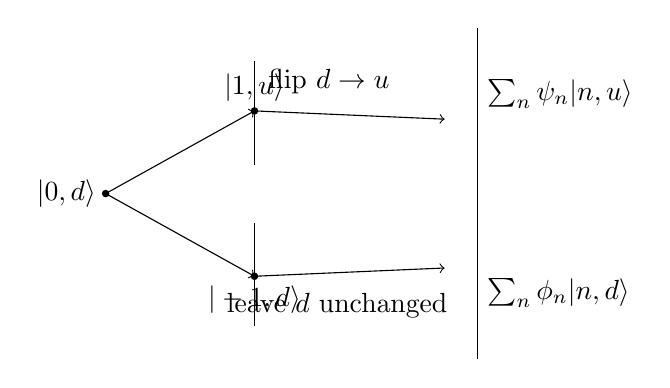
\begin{tikzpicture}[scale=1.05]
\fill (0,0) circle (1.3pt);
\node[left] at (0,0) {$|0,d\rangle$};

\draw (1.8,1.6) -- (1.8,0.35);
\draw (1.8,-0.35) -- (1.8,-1.6);
\fill (1.8,1) circle (1.3pt);
\fill (1.8,-1) circle (1.3pt);
\node[above] at (1.8,1) {$|1,u\rangle$};
\node[below] at (1.8,-1) {$|-1,d\rangle$};

\draw (4.5,2.0) -- (4.5,-2.0);
\node[right] at (4.5,1.2) {$\sum_n \psi_n |n,u\rangle$};
\node[right] at (4.5,-1.2) {$\sum_n \phi_n |n,d\rangle$};

\draw[->] (0,0) -- (1.8,1);
\draw[->] (0,0) -- (1.8,-1);
\draw[->] (1.8,1) -- (4.1,0.9);
\draw[->] (1.8,-1) -- (4.1,-0.9);

\node at (2.7,1.35) {flip \(d\to u\)};
\node at (2.8,-1.35) {leave \(d\) unchanged};
\end{tikzpicture}
\caption{검출기 스핀과의 얽힘으로 나타낸 측정. 위쪽 경로는 장치의 스핀을 뒤집고, 아래쪽 경로는 스핀을 그대로 둡니다.}
\end{figure}

강의에서 가정한 대로 스크린까지 가는 동안 스핀에 더 이상 아무 일도 일어나지 않는다고 합시다. 그러면
\begin{align}
|1,u\rangle &\longrightarrow \sum_n \psi_n |n,u\rangle, \\
|-1,d\rangle &\longrightarrow \sum_n \phi_n |n,d\rangle.
\end{align}
따라서 두 슬릿을 모두 열었을 때의 최종 상태는
\begin{equation}
|\Psi_{\mathrm{final}}\rangle
  = \sum_n \psi_n |n,u\rangle + \sum_n \phi_n |n,d\rangle.
\end{equation}
이것은 전자 하나만의 상태를 중첩한 것이 아닙니다. 전자와 장치가 이루는 얽힌 상태입니다.

\begin{figure}[htbp]
\centering
\includegraphics[width=0.68\textwidth]{lecture_06_figure_13.png}
\caption{두 경로의 진폭은 서로 직교하는 장치 기록을 지닌 채 스크린에 도달합니다.}
\lectureframe{01:47:35}
\end{figure}

지점 \(m\)에 도달할 확률을 계산하는 가장 간단한 방법은 전자 부분계에서 그 지점에 대한 사영 연산자를 사용하는 것입니다.
\begin{equation}
\Pi_m = |m\rangle\langle m|\otimes I_{\mathrm{spin}}.
\end{equation}
최종 상태에 \(\Pi_m\)를 적용하면
\begin{equation}
\Pi_m |\Psi_{\mathrm{final}}\rangle
= |m\rangle\bigl(\psi_m|u\rangle+\phi_m|d\rangle\bigr).
\end{equation}
따라서 \(m\)에 도달할 확률은
\begin{align}
P_m
  &= \langle \Psi_{\mathrm{final}}|\Pi_m|\Psi_{\mathrm{final}}\rangle \\
  &= \bigl(\psi_m^*\langle u|+\phi_m^*\langle d|\bigr)
     \bigl(\psi_m|u\rangle+\phi_m|d\rangle\bigr) \\
  &= |\psi_m|^2 + |\phi_m|^2
     + \psi_m^*\phi_m\langle u|d\rangle
     + \phi_m^*\psi_m\langle d|u\rangle.
\end{align}
그러나 기록 상태들은 서로 직교합니다.
\begin{equation}
\langle u|d\rangle=0.
\end{equation}
그러므로 교차항은 사라집니다.
\begin{equation}
P_m = |\psi_m|^2 + |\phi_m|^2.
\end{equation}
이것이 강의에서 제시하는 수학적 핵심입니다. 경로 정보가 기록되면 간섭은 사라지고 확률은 고전적인 방식으로 더해집니다.

\begin{classroomqa}
\lecturetimestamp{01:49:09}
\audiencequestion{중첩 \(|1\rangle+|-1\rangle\)과 상태 \(|1,u\rangle+|-1,d\rangle\)은 어떻게 다른가요?}
\lecturerresponse{첫 번째는 두 위치의 선형 결합으로 표현되는 하나의 계에 관한 것입니다. 그 계와 얽힐 다른 것은 없습니다. 두 번째는 두 계에 관한 것으로, 경로와 검출기 스핀을 서로 상관시킵니다. 따라서 스핀을 읽으면 경로에 관한 정보를 알 수 있습니다.}
\end{classroomqa}

\section{환경에 남는 기록과 부분 측정}

의도적으로 만든 검출기만이 기록을 남기는 것은 아닙니다. 슬릿 근처의 원자, 잔류 기체, 열을 띤 표면, 또는 다른 자유도도 경로와 상관될 수 있습니다. 그 최종 상태가 \(|E_1\rangle\)와 \(|E_2\rangle\)라면 경로 상태는 다음과 같은 형태가 됩니다.
\begin{equation}
|\Psi\rangle
=\sum_n\left(\psi_n|n\rangle|E_1\rangle
+\phi_n|n\rangle|E_2\rangle\right).
\end{equation}
이제 간섭 항에는 겹침 정도 \(\langle E_1|E_2\rangle\)가 곱해집니다. 직교하는 기록은 경로를 완전히 구별할 수 있게 하므로 간섭을 완전히 없앱니다. 기록이 동일하면 \(\langle E_1|E_2\rangle=1\)가 되어 간섭이 보존됩니다. 겹침이 그 중간이면 가시도도 부분적으로 남습니다.

\begin{figure}[htbp]
\centering
\includegraphics[width=0.68\textwidth]{lecture_06_figure_14.png}
\caption{서로 겹치는 환경 파동 묶음과 분리된 환경 파동 묶음은 부분적인 경로 기록과 완전한 경로 기록을 보여 줍니다.}
\lectureframe{01:53:40}
\end{figure}

\begin{classroomqa}
\lecturetimestamp{01:50:48}
\audiencequestion{슬릿 근처에 있는 보통의 원자도 누군가 의도적으로 관측하지 않더라도 지나가는 전자와 얽힐 수 있나요?}
\lecturerresponse{그렇습니다. 작용하는 것은 지식이 아니라 물리적 상관관계입니다. 원자나 주변 기체가 충분히 교란되어 나중 상태로 경로를 구별할 수 있게 되면, 경로 정보를 기록하고 간섭을 억제합니다. 그래서 이런 실험에는 차폐와 낮은 온도가 필요하며, 광자처럼 상호작용이 약한 입자를 쓰는 경우도 많습니다.}
\end{classroomqa}

냉각하면 환경의 자유도들이 바닥 상태에 가까워져 우발적인 기록이 줄어듭니다. 에너지 간격도 도움이 됩니다. 입사 입자가 최소 들뜸 에너지를 공급할 수 없다면, 환경은 경로 정보를 보존하지 못할 수 있습니다. 반대로 하전 입자는 전기장을 통해 주변 물질을 교란할 수 있으므로, 전자 간섭 실험은 특히 까다롭습니다.

\begin{classroomqa}
\lecturetimestamp{01:54:49}
\audiencequestion{전자 하나씩으로도 정말 간섭 무늬를 얻을 수 있나요?}
\lecturerresponse{전자 하나는 국소화된 검출 흔적 하나만 남깁니다. 입자들이 서로 상호작용하지 않도록 충분한 간격을 두고 한 번에 하나씩 보내 여러 번 반복합니다. 이렇게 누적된 빈도 분포에서 간섭 무늬가 나타납니다. 한 번의 사건만으로는 작은 흔적 하나만 얻을 뿐입니다.}
\end{classroomqa}

\begin{classroomqa}
\lecturetimestamp{01:55:59}
\audiencequestion{측정은 얽힘을 없애나요, 아니면 만들어 내나요?}
\lecturerresponse{경로를 구별하는 상호작용은 계와 장치 사이에 얽힘을 만들고, 그 얽힘은 각 경로 사이의 간섭을 없앱니다. 이후의 측정은 장치와 또 다른 계를 상관시킬 수 있으며, 그에 따라 나머지 상태를 조건부로 정할 수도 있습니다. 따라서 어떤 두 부분계와 어떤 간섭을 말하는지 항상 분명히 해야 합니다.}
\end{classroomqa}

\begin{classroomqa}
\lecturetimestamp{01:57:44}
\audiencequestion{상호작용을 약하게 해서 장치가 경로 정보를 일부만 얻도록 할 수 있나요?}
\lecturerresponse{그렇습니다. 약한 상호작용에서는 어떤 진폭으로만 검출기가 뒤집혀, 서로 직교하지 않는 기록 상태들이 남을 수 있습니다. 그러면 경로는 부분적으로만 구별되고 간섭도 일부만 줄어듭니다. 측정이 강할수록 구별 가능성이 커지고 기록과의 얽힘은 강해지며 무늬의 가시도는 낮아집니다.}
\end{classroomqa}

따라서 여기서 말하는 붕괴는 구체적으로, 경로 정보가 다른 계에 기록될 때 교차항이 사라지는 현상이다. 기록이 없으면 진폭이 더해진다. 기록들이 완전히 구별 가능하면 기록 상태들의 내적은 영이 되고 확률이 더해진다. 이 두 극한 사이에서는 측정 강도와 간섭 가시도가 연속적으로 변한다.
